\chapter{Heap \label{ch:heap}}
\section{Introduzione}
L'heap è una struttura dati basata sull'albero i cui nodi rispettano una particolare proprietà e condividono delle relazioni. Vi sono due tipi di heap: min-heap e max-heap. In questo capitolo verranno indagati i max-heap \cite{cormen2022introduction}, la loro rappresentazione e le procedure fondamentali che permettono di costruirli e mantenerli. La complessità temporale di una di queste operazioni servirà da termine di paragone per la versione quantistica di questa stessa operazione.

Un max-heap è un albero binario quasi completo, ossia un albero binario in cui ogni livello è completamente riempito ad eccezione, eventualmente, dell'ultimo, che viene riempito da sinistra verso destra. Questa struttura viene tipicamente rappresentata tramite un array $A$, dove ogni nodo dell'albero corrisponde ad un elemento dell'array e le relazioni di parentela tra i nodi sono espresse tramite semplici operazioni aritmetiche sugli indici.

\section{Proprietà \label{sec:proprieta}}
Per tutti i nodi, ad eccezione della radice, è vero che:
\begin{equation}
  A[\text{Parent}(i)] \geq A[i]
\end{equation}
Questa relazione è detta proprietà di max-heap: il valore contenuto in un nodo è sempre maggiore o uguale al valore dei suoi figli. Ne consegue, per transitività, che l'elemento massimo dell'intera struttura si trova sempre in corrispondenza della radice dell'albero, cioè in $A[0]$.

Definiamo l'altezza di un nodo in un heap come la lunghezza del percorso discendente più lungo dal nodo ad una foglia. Si afferma perciò che l'altezza di un heap è uguale all'altezza della sua radice. Poiché l'heap è un albero binario completo o quasi completo con $n$ nodi, la sua altezza è $\mathcal{O}(\log n)$; questa proprietà è cruciale, in quanto la maggior parte delle procedure fondamentali sull'heap opera seguendo un singolo cammino dalla radice ad una foglia (o viceversa), ottenendo così una complessità logaritmica rispetto al numero di elementi.

\section{Figli \label{sec:figli}}
È possibile computare la posizione di padre, figlio sinistro e destro di un nodo qualsiasi data la sua posizione $i$.
\lstset{stringstyle=\ttfamily}
\begin{lstlisting}[caption={Operazioni},label=lst:multicorrelation]
Left(i)
  return (i << 1) | 1
Right(i)
  return (i + 1) << 1
Parent(i)
  return (i - 1) >> 1
\end{lstlisting}
Indicizzando l'array $A$ a partire da $0$, queste operazioni permettono di navigare l'albero senza bisogno di puntatori espliciti: dato un nodo in posizione $i$, i suoi figli si trovano rispettivamente in posizione $2i + 1$ e $2i + 2$, mentre il padre si trova in posizione $\lfloor (i-1)/2 \rfloor$.

\begin{figure}[h]
  \centering
  
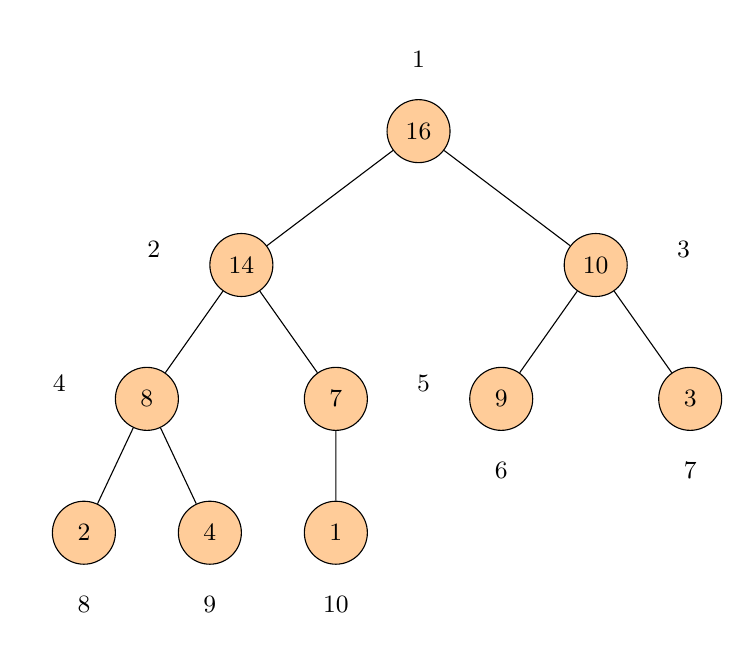
\begin{tikzpicture}[
    every node/.style={circle, draw, fill=orange!40, minimum size=8mm, font=\small},
    level distance=17mm,
    level 1/.style={sibling distance=45mm},
    level 2/.style={sibling distance=24mm},
    level 3/.style={sibling distance=16mm},
    edge from parent/.style={draw, -}
  ]

  \node[label={[yshift=1mm]above:1}] (n1) {16}
  child { node[label={[xshift=-3mm,yshift=2mm]left:2}] (n2) {14}
      child { node[label={[xshift=-3mm,yshift=2mm]left:4}] (n4) {8}
          child { node[label={[yshift=-1mm]below:8}] (n8) {2} }
          child { node[label={[yshift=-1mm]below:9}] (n9) {4} }
        }
      child { node[label={[xshift=3mm,yshift=2mm]right:5}] (n5) {7}
          child { node[label={[yshift=-1mm]below:10}] (n10) {1} }
        }
    }
  child { node[label={[xshift=3mm,yshift=2mm]right:3}] (n3) {10}
      child { node[label={[yshift=-1mm]below:6}] (n6) {9} }
      child { node[label={[yshift=-1mm]below:7}] (n7) {3} }
    };

\end{tikzpicture}
\hspace{2cm}
% ==============================================
% Figura (b): Rappresentazione ad array con archi
% ==============================================
\begin{tikzpicture}[
    every node/.style={draw, minimum width=8mm, minimum height=8mm, font=\small},
    node distance=0mm
  ]

  % Valori dell'array
  \node (a1) {16};
  \node[right=of a1] (a2) {14};
  \node[right=of a2] (a3) {10};
  \node[right=of a3] (a4) {8};
  \node[right=of a4] (a5) {7};
  \node[right=of a5] (a6) {9};
  \node[right=of a6] (a7) {3};
  \node[right=of a7] (a8) {2};
  \node[right=of a8] (a9) {4};
  \node[right=of a9] (a10) {1};

  % Indici sopra, ben distanziati dagli archi
  \foreach \i in {1,...,10}{
      \node[draw=none, above=7mm of a\i, font=\small] {\i};
    }

  % Archi genitore-figlio: curvatura proporzionale alla distanza tra i nodi
  % padre 1 -> figli 2,3
  \draw[-{Latex[length=2mm]}] (a1.north) to[bend left=25] (a2.north);
  \draw[-{Latex[length=2mm]}] (a1.north) to[bend left=45] (a3.north);

  % padre 2 -> figli 4,5
  \draw[-{Latex[length=2mm]}] (a2.north) to[bend left=25] (a4.north);
  \draw[-{Latex[length=2mm]}] (a2.north) to[bend left=45] (a5.north);

  % padre 3 -> figli 6,7
  \draw[-{Latex[length=2mm]}] (a3.north) to[bend left=25] (a6.north);
  \draw[-{Latex[length=2mm]}] (a3.north) to[bend left=45] (a7.north);

  % padre 4 -> figli 8,9
  \draw[-{Latex[length=2mm]}] (a4.north) to[bend left=25] (a8.north);
  \draw[-{Latex[length=2mm]}] (a4.north) to[bend left=45] (a9.north);

  % padre 5 -> figlio 10
  \draw[-{Latex[length=2mm]}] (a5.north) to[bend left=45] (a10.north);

\end{tikzpicture}
  \caption{Rappresentazione di un max-heap come albero e come array.}
\end{figure}

\section{Procedure \label{sec:procedure}}
\subsection{Max-Heapify}
La procedura Max-Heapify ha il compito di mantenere la proprietà di max-heap. Riceve in input un array $A$ e un indice $i$ e assume che i sottoalberi radicati in $\text{Left}(i)$ e $\text{Right}(i)$ siano già degli heap validi, mentre $A[i]$ potrebbe violare la proprietà rispetto ai suoi figli. La procedura fa "scendere" il valore $A[i]$ lungo l'albero fino a ripristinare la proprietà di heap:
\begin{lstlisting}[caption={Max-Heapify},label=lst:max-heapify,escapechar=|]
Max-Heapify(A, i)
  l = Left(i)
  r = Right(i)
  if l < A.heap-size and A[l] > A[i]
    largest = l
  else
    largest = i
  if r < A.heap-size and A[r] > A[largest]
    largest = r
  if largest != i
    exchange A[i] with A[largest]
    Max-Heapify(A, largest)
\end{lstlisting}

Intuitivamente, il procedimento consiste nel trascinare giù il nodo $A[i]$: si confronta il valore corrente con quello dei due figli e, se uno dei due è maggiore, lo si scambia con il valore in posizione $i$, ripetendo poi il confronto nella posizione in cui il valore originario si è spostato, finché non si raggiunge una posizione in cui la proprietà è rispettata rispetto a entrambi i figli, o una foglia. Ad ogni chiamata ricorsiva, il nodo scende di un livello lungo l'albero; poiché l'altezza dell'heap è $\mathcal{O}(\log n)$, la complessità di Max-Heapify è $\mathcal{O}(\log n)$.

\subsection{Build-Max-Heap}
La procedura Build-Max-Heap costruisce un max-heap valido a partire da un array non ordinato, applicando Max-Heapify a tutti i nodi non foglia, procedendo dal basso verso l'alto:
\begin{lstlisting}[caption={Build-Max-Heap},label=lst:build-max-heap]
Build-Max-Heap(A)
  A.heap-size = A.length
  for i = floor(A.length / 2 - 1) downto 0
    Max-Heapify(A, i)
\end{lstlisting}
Applicando Max-Heapify dal basso verso l'alto, la procedura garantisce che, quando viene chiamata su un nodo $i$, i suoi due sottoalberi siano già heap validi cosicché al termine dell'intero ciclo l'intero array soddisfi la proprietà di max-heap.

Si osserva che, sebbene ogni singola chiamata a Max-Heapify costi $\mathcal{O}(\log n)$ nel caso peggiore, il costo complessivo di Build-Max-Heap è in realtà $\mathcal{O}(n)$ e non $\mathcal{O}(n \log n)$. Questo risultato si giustifica osservando che il costo di Max-Heapify su un nodo dipende non dall'altezza dell'intero heap, ma dall'altezza $h$ del nodo specifico su cui viene invocata: in un albero binario quasi completo con $n$ nodi, al più $\lceil n/2^{h+1}\rceil$ nodi si trovano ad altezza $h$, e la maggior parte dei nodi si trova infatti nei livelli più bassi (a piccola altezza), dove Max-Heapify costa poco. Il costo complessivo è pertanto limitato da \cite{cormen2022introduction}:
\begin{equation}
  \sum_{h=0}^{\lfloor \log_2 n \rfloor} \left\lceil \frac{n}{2^{h+1}} \right\rceil \mathcal{O}(h) = \mathcal{O}\left(n \sum_{h=0}^{\infty} \frac{h}{2^h}\right).
\end{equation}
Poiché la serie $\sum_{h=0}^{\infty} h/2^h$ converge al valore $2$, il costo complessivo di Build-Max-Heap è $\mathcal{O}(n)$.

\subsection{Verifica della proprietà}
Oltre alla costruzione, è utile considerare il problema, concettualmente più semplice, di verificare se un array $A$ già dato soddisfi la proprietà di max-heap. A differenza di Max-Heapify, questa procedura non modifica l'array, ma si limita a confrontare ciascun nodo interno con i propri figli, restituendo un esito booleano:
\begin{lstlisting}[caption={Verify-Max-Heap},label=lst:verify-max-heap]
Verify-Max-Heap(A)
  for i = 0 to floor(A.length / 2) - 1
    l = Left(i)
    r = Right(i)
    if A[i] < A[l]
      return false
    if r < A.length and A[i] < A[r]
      return false
  return true
\end{lstlisting}
La procedura esamina, uno alla volta, tutti i $\lfloor n/2 \rfloor$ nodi interni dell'heap, eseguendo per ciascuno un numero costante di confronti. Nel caso peggiore, ossia quando l'array soddisfa effettivamente la proprietà, oppure quando l'unica violazione si trova nell'ultimo nodo interno esaminato, è necessario esaminare tutti i nodi interni, per cui la complessità è $\Theta(n)$; nel caso migliore, in cui la prima violazione si trova già nel primo nodo esaminato, la complessità si riduce a $\mathcal{O}(1)$.

Questo risultato costituisce il termine di paragone classico rispetto al quale valutare l'approccio quantistico proposto nei capitoli successivi: individuare un singolo nodo che violi la proprietà, nel caso peggiore, richiede classicamente di esaminare linearmente tutti i nodi interni, mentre l'algoritmo di Grover applicato allo stesso problema promette, in linea di principio, un vantaggio quadratico nel numero di chiamate all'oracolo di verifica.